%!TEX root = ../template.tex
%%%%%%%%%%%%%%%%%%%%%%%%%%%%%%%%%%%%%%%%%%%%%%%%%%%%%%%%%%%%%%%%%%%%
%% chapter5.tex
%% NOVA thesis document file
%%
%% Chapter with lots of dummy text
%%%%%%%%%%%%%%%%%%%%%%%%%%%%%%%%%%%%%%%%%%%%%%%%%%%%%%%%%%%%%%%%%%%%

\typeout{NT FILE chapter6.tex}%

\chapter{Related Work}
\label{cha:related_work}

\section{Introduction}
In this chapter, we will explore existing pedagogical tools for teaching Formal Languages and Automata Theory (FLAT), 
including ones that provide support for finite-state transducers (FSTs). As well as comparing them with each other, and with the OFLAT tool. 
This is done in order to contextualize the work to be done.

\section{JFLAP: Java Formal Languages and Automata Package}

JFLAP (Java Formal Languages and Automata Package)\cite{JFLAP} is a widely adopted educational tool for teaching and learning formal languages and automata theory. 
Initially developed in the 1990s by Professor Susan H. Rodger and her students at Rensselaer Polytechnic Institute, JFLAP was first created in C++ and X Window under the name FLAP. 
It was later rewritten in Java and renamed JFLAP, enhancing its portability and usability. As a Java application, it runs on most systems equipped with the Java Runtime Environment (JRE).

JFLAP offers a comprehensive suite of features supporting the construction, simulation, testing, and conversion of theoretical models. 
Users can interactively design deterministic and non-deterministic finite automata, draw state diagrams, define transitions based on input symbols, and specify start and accept states. 
The tool provides immediate visual feedback by allowing users to simulate automata step by step, highlighting state transitions and input consumption. 
Figure~\ref{fig:JFLAPModels} illustrates the model option in JFLAP.

\begin{figure}[H]
  \centering
  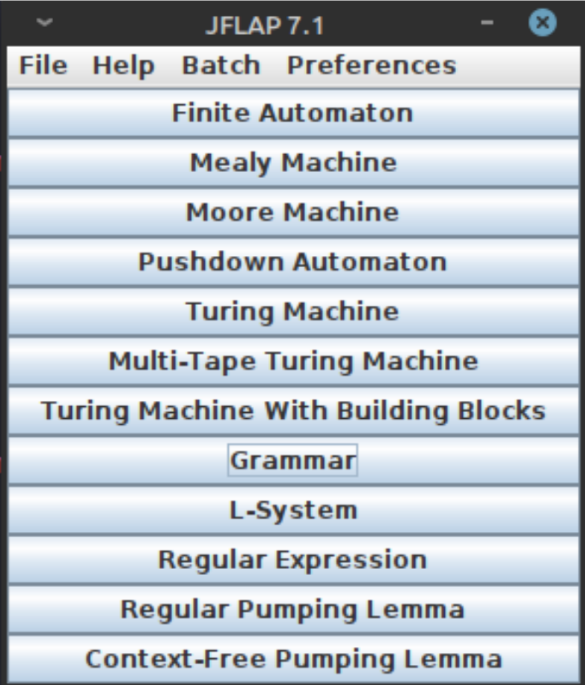
\includegraphics[width=0.5\textwidth]{JFLAPModels.png}
  \caption{Model list available in JFLAP.}
  \label{fig:JFLAPModels}
\end{figure}

JFLAP also offers support for finite-state transducers, it has simulation and visualization of Mealy and Moore machines, allowing users
to observe state transitions alongside produced outputs.
Figure~\ref{fig:jflap-mealy} shows a simple Mealy machine in JFLAP,.

\begin{figure}[H]
  \centering
  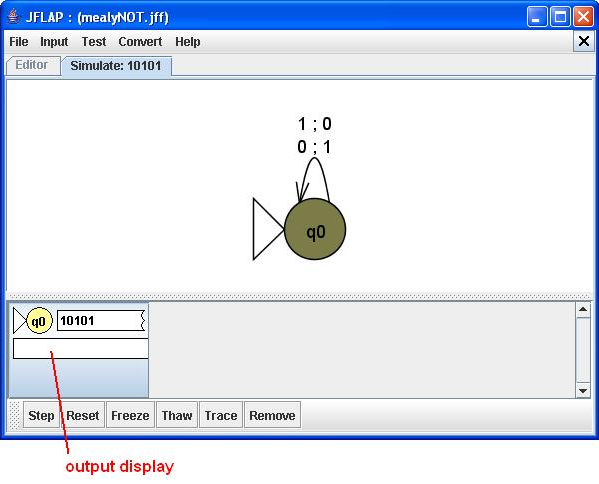
\includegraphics[width=0.7\textwidth]{jflap-mealy.png}
  \caption{A simple Mealy machine in JFLAP.}
  \label{fig:jflap-mealy}
\end{figure}

This example consists of a single state, \texttt{q0}, which serves as both the initial and active state throughout the computation. 
The transitions are labeled in the form \texttt{input ; output}, indicating that an input of \texttt{1} produces an output of \texttt{0}, 
and vice versa. The input string \texttt{10101} is provided below the state diagram, and the machine's output is displayed dynamically as the simulation progresses. 
The interface includes a control panel with options such as \texttt{Step}, \texttt{Reset}, \texttt{Trace}, and others, allowing users to simulate the machine step-by-step.


Beyond automata, JFLAP supports formal grammar manipulation, including regular, context-free, and unrestricted grammars. 
It can convert between NFAs, regular expressions, and grammars, illustrating their equivalence.

\subsubsection*{Conclusion}
JFLAP distinguishes itself as one of the most complete and pedagogically effective tools in formal language education. 
It supports a wide variety of computational models and conversions grounded in formal theory. 

\section{FAdo}
Similar to OFLAT, FAdo\cite{FAdo} is a Portuguese project that aims to develop an interactiv environment for the symbolic manipulation of formal languages. 
It however relies on a Python library designed for symbolic manipulation of finite automata and regular expressions. 
It supports both deterministic and nondeterministic finite automata, 
providing minimization, equivalence checking, language operations 
(union, intersection, complementation), and conversion between automata and regular expressions.

In contrast to interactive graphical tools such as JFLAP, OFLAT, and Automaton Simulator, the notion of acceptance in FAdo is more limited in scope, 
particularly with regard to visualization and user interaction. 
FAdo is primarily intended to be used programmatically within a Python interpreter or in script-based workflows. 
As such, it does not provide a graphical user interface or native support for animated, step-by-step execution of automata.
Instead, the FAdo library emphasizes flexibility and extensibility within a code-based environment. 
To determine whether a word is accepted by a defined finite automaton, users can invoke the method evalWord(word), 
which simply returns a Boolean value (True or False). 
This binary output informs whether the automaton, in its current configuration, accepts the given input string. 
While this functionality is effective for bulk testing or automated workflows, 
it does not provide insight into how the automaton processes the string or transitions through its states during evaluation.
For users who wish to simulate the acceptance process manually, FAdo provides a lower-level function, evalSymbol(init, symb). 
This function allows for inspection of individual transitions by returning the resulting state reached when consuming a symbol symb from a current state init. 
By iteratively applying evalSymbol for each symbol in the input string—updating 
the initial state to be the result of the previous call—a user can effectively simulate the path that the automaton takes through its states.
However, this manual step-by-step execution is not integrated into the library as a built-in feature.
In educational contexts, this limitation makes FAdo less suited for beginners or for visual demonstrations of automaton behavior. 
However, its strength lies in its integration into Python's ecosystem, which enables programmatic construction, manipulation, and analysis of automata and formal languages, 
making it a powerful tool for advanced users, researchers, or developers building larger systems that rely on formal language processing.

\section{Automaton Simulator}

The Automaton Simulator\cite{automatonSimulator} is an open-source, browser-based tool designed for constructing and simulating various types of finite automata. 
It supports deterministic finite automata (DFA), nondeterministic finite automata (NFA), and pushdown automata (PDA), 
that offers a simple and interactive environment for educational purposes.

The interface is divided into several functional sections that enhance usability. 
On the left-hand side Figure~\ref{fig:automaton-simulator-left-panel}, users can input strings for testing. 
There are two main boxes: one labeled \texttt{Accept (one per line)} for input strings expected to be accepted by the automaton, 
and one labeled \texttt{Reject (one per line)} for strings expected to be rejected. 
These strings can be tested in bulk using the \textit{Bulk Testing} feature, which evaluates all entries at once and displays their acceptance or rejection.
There is also a \texttt{Test/Debug} field, which allows for dynamic simulation.

\begin{figure}[H]
  \centering
  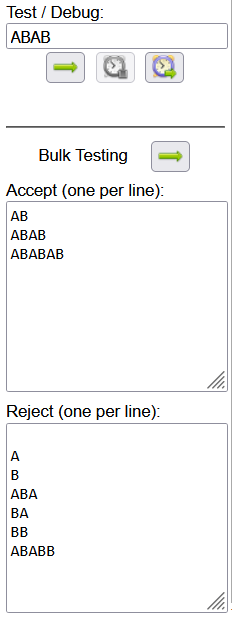
\includegraphics[width=0.3\textwidth]{ASLeft.png}
  \caption{Left panel of the Automaton Simulator.}
  \label{fig:automaton-simulator-left-panel}
\end{figure}

Below these input areas is the \texttt{Test Results} panel, where detailed feedback is shown after the test runs. 
Above the input section, buttons for loading, saving, and resetting the automaton are displayed. 
The central canvas of the interface is where the automaton is constructed Figure~\ref{fig:automaton-simulator-center}. States are created by clicking, and transitions are added by clicking and dragging between states. 
The simulation highlights the current state using a different color, the transition being taken, and the unprocessed portion of the input string. 
This is especially useful in step-by-step simulations where the learner can observe the exact sequence of transitions being executed.

Each state is displayed as a rounded rectangle, with different markings to indicate its role:
\begin{itemize}
  \item A checked box denotes an accepting (final) state.
  \item Transitions are labeled with the input symbol that triggers them.
\end{itemize}

The simulator provides feedback on acceptance using textual cues such as "Accepted" or "Rejected", displayed near the top-left corner of the interface. 
During step-by-step execution, this feedback updates in real time as the input string is consumed.

\begin{figure}[H]
  \centering
  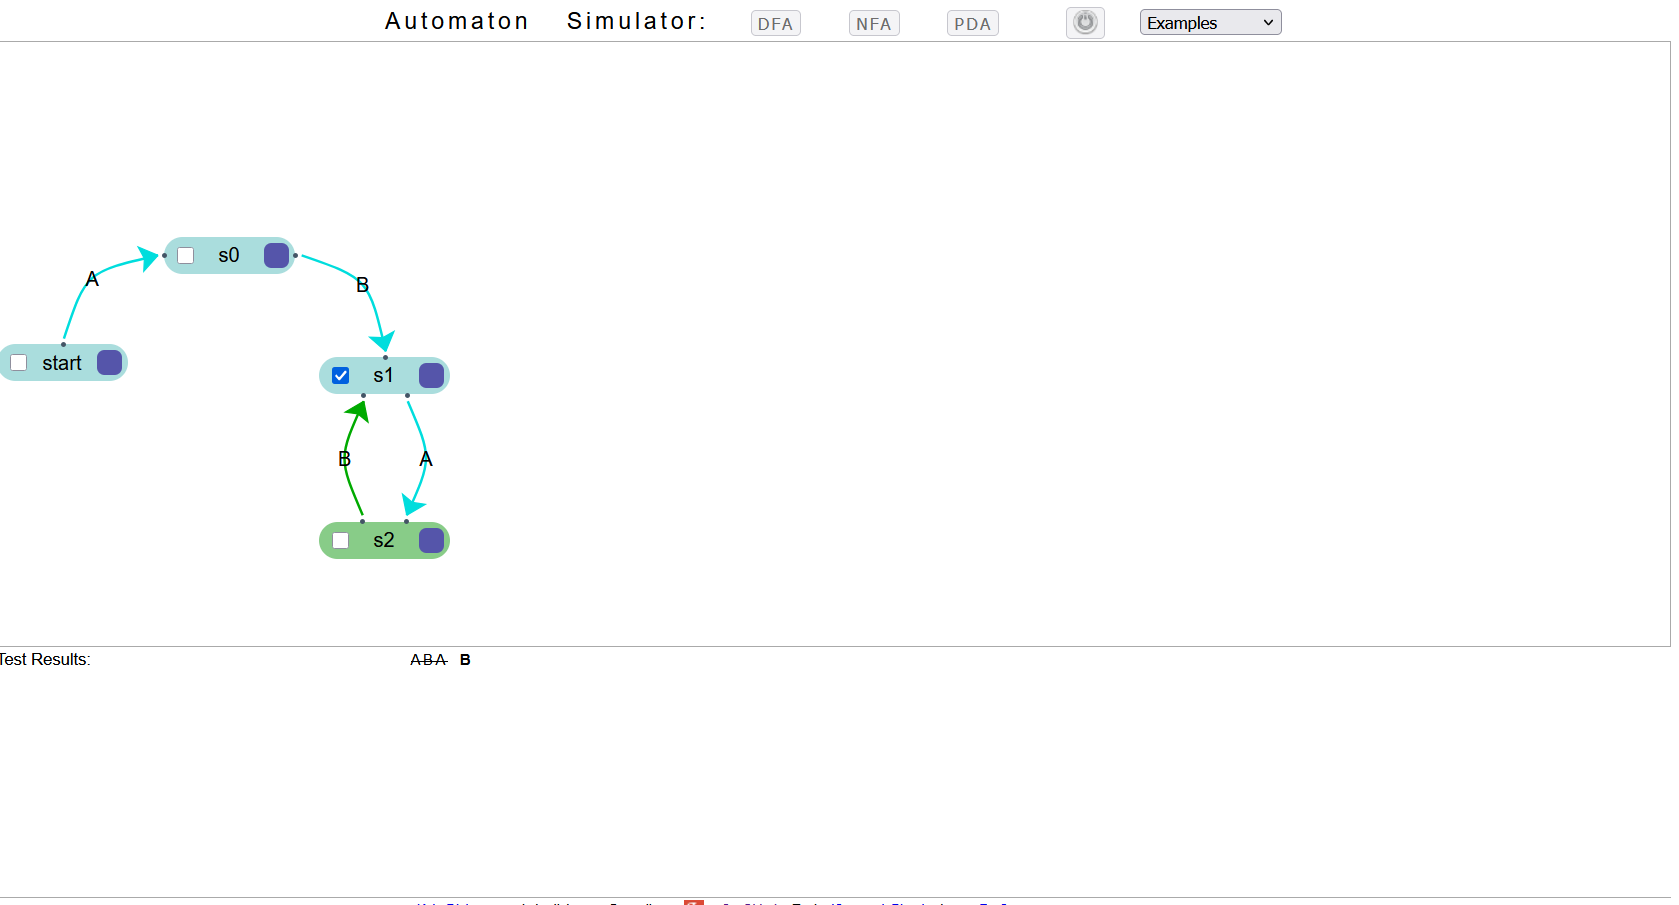
\includegraphics[width=0.95\textwidth]{ASCenter.png}
  \caption{Central area of the Automaton Simulator.}
  \label{fig:automaton-simulator-center}
\end{figure}

\subsubsection*{Conclusion}

The Automaton Simulator provides an effective and user-friendly platform for constructing and simulating finite automata directly in the web browser. 
Its strength lies in its simplicity and immediate feedback mechanism, which makes it ideal for introductory coursework or quick validation of automaton logic.
Although it lacks the extensive model coverage and transformation tools found in more comprehensive platforms like JFLAP or OFLAT, 
it fills a useful niche as a lightweight and accessible teaching aid. When used alongside these more feature-rich systems, 
the Automaton Simulator contributes to a diverse and flexible pedagogical toolkit for exploring the foundational principles of automata theory.


\section{Flap.js}
Flap.JS is a web application therefore easily available on all kinds of devices, including mobile
devices. It supports the graphical creation of Finite Automata, Regular Expressions, and
Pushdown Automata, as well as tests and conversions, but none of these use animations, which would improve the
learning process.
In there web application, we can see that support for finite state transducers is not available, however,
mealy machines, moore machines and turing machines are greyed out, indicating that they are planned features to be added in the future.

This makes Flap.js a tool that while is still under development, but it has the potential to become a powerful educational tool for FLAT.
However, as it stands, it does not provide as much variety in its current state as some of the others, like JFLAP and our OFLAT. As well as having a less intuitive interface,
then Automaton Simulator, which is simpler and provides similar functionalities.

% \lipsum[1-100]
% \lipsum[1-700]
% \lipsum[1-700]
% \lipsum[1-700]
% \lipsum[1-700]
% \lipsum[1-700]
% \lipsum[1-700]
% \lipsum[1-700]
% \lipsum[1-700]
